% Chapter Template

\chapter{Diseño e Implementación} % Main chapter title

\label{Chapter3} % Change X to a consecutive number; for referencing this chapter elsewhere, use \ref{ChapterX}

En el siguiente capítulo se presentará el diseño y la implementación de las tres partes fundamentales del equipo. Se abarcarán aspectos de hardware, firmware y diseño mecánico.
%----------------------------------------------------------------------------------------
%	SECTION 1
%----------------------------------------------------------------------------------------
\section{Hardware}
\subsection{Diseño basado en módulos de hardware libre}

Para el diseño del hardware se utilizó el software libre de diseño de circuitos impresos KICAD \citep{web_kicad}, que en sus últimas versionas presentá mejoras significativas respecto a sus predecesoras.

El diseño de la placa electrónica se baso en el estudio de los siguientes módulos:

\begin{itemize}
\item Módulo NodeMCU \citep{web_nodemcu}
\item TMC5130-EVAL \citep{3_web_trinamic_placa}	
\end{itemize}

Se destaca que ambos proyectos adhieren a la filosofía del hardware libre por lo tanto se pudieron descargar y estudiar los diagramas esquemáticos de ambas placas. 


El módulo NodeMCU en una placa de desarrollo que contiene el SoC ESP32-WROOM, cuenta también con un conversor SERIAL-USB que permite conectar el módulo directamente a un puerto USB de computadora. Permitiendo de esta manera descargar el firmware sin necesidad de contar con un programador externo.
El la imagen 

\ref{fig:dip_3d_model}


\begin{figure}[htbp]
	\centering
	\includegraphics[width=.8\textwidth]{./Figures/kicad_conversor.png}
	\caption{Conversor UART-USB.}
	\label{fig:kicad_conversor}
\end{figure}

\begin{figure}[htbp]
	\centering
	\includegraphics[width=.5\textwidth]{./Figures/kicad_clock.png}
	\caption{Clock para el CI TMC5130.}
	\label{fig:kicad_clock}
\end{figure}

\begin{figure}[htbp]
	\centering
	\includegraphics[width=.6\textwidth]{./Figures/kicad_esp.png}
	\caption{Módulo ESP32.}
	\label{fig:kicad_esp}
\end{figure}

\begin{figure}[htbp]
	\centering
	\includegraphics[width=.8\textwidth]{./Figures/kicad_tension.png}
	\caption{Módulo de entrada.}
	\label{fig:kicad_tension}
\end{figure}
 
\begin{figure}[htbp]
	\centering
	\includegraphics[width=0.8\textwidth]{./Figures/kicad_trinamic.png}
	\caption{CI TMC5130.}
	\label{fig:kicad_trinamic}
\end{figure} 
 
 
 
 
Finalmente podemos observar en la figura \ref{fig:dip_3d_model} el diseño 3D generado por el software KICAD. La placa cuenta con licencia CERN OHL v.1.2 \citep{web_cern_licence}.


\begin{figure}[htbp]
	\centering
	\includegraphics[width=.5\textwidth]{./Figures/dip_3d_model.pdf}
	\caption{Modelo 3D Kicad.}
	\label{fig:dip_3d_model}
\end{figure}
         



  
%-----------------------------------
%	SUBSECTION 1
%-----------------------------------
\subsection{Fabricación}
%-----------------------------------
%	SUBSECTION 2
%-----------------------------------
La placa electrónica se fabricó con el proveedor local de circuitos impresos Ernesto Mayer S.A. \citep{web_mayer}. A continuación se presenta la información de diseño de la placa y de describen algunas  restricciones de diseños impuestas por el fabricante:

\begin{itemize}

\item Grilla de posicionamiento principal: 0.25mm
\item Grilla de ruteo principal: 0.25mm
\item Agujeros de montaje: 3.2mm
\item Pistas principales: 0.5mm
\item Pistas inferiores: 0.25mm (límite particular 8mils(0.20mm))
\item Pistas superiores: 0.8mm
\item Vías: 0.8mm/0.4mm (límite particular 8mils(0.20mm))
\item Margen general: 0.22 mm
\item Margen particular: 0.2 mm (límite particual 8 mils(0.20mm))
\item Fabricación: espesor 1.6mm FR4  
\item Restricciones generales del fabricante: estándar 10 mils

\end{itemize}

Luego de fabricar el PCB, se continuó con el todo el montaje de componentes electrónicos superficiales que estuvo a cargo de la empresa Asembli S.A. \citep{web_asembli}.


\begin{figure}[htbp]
	\centering
	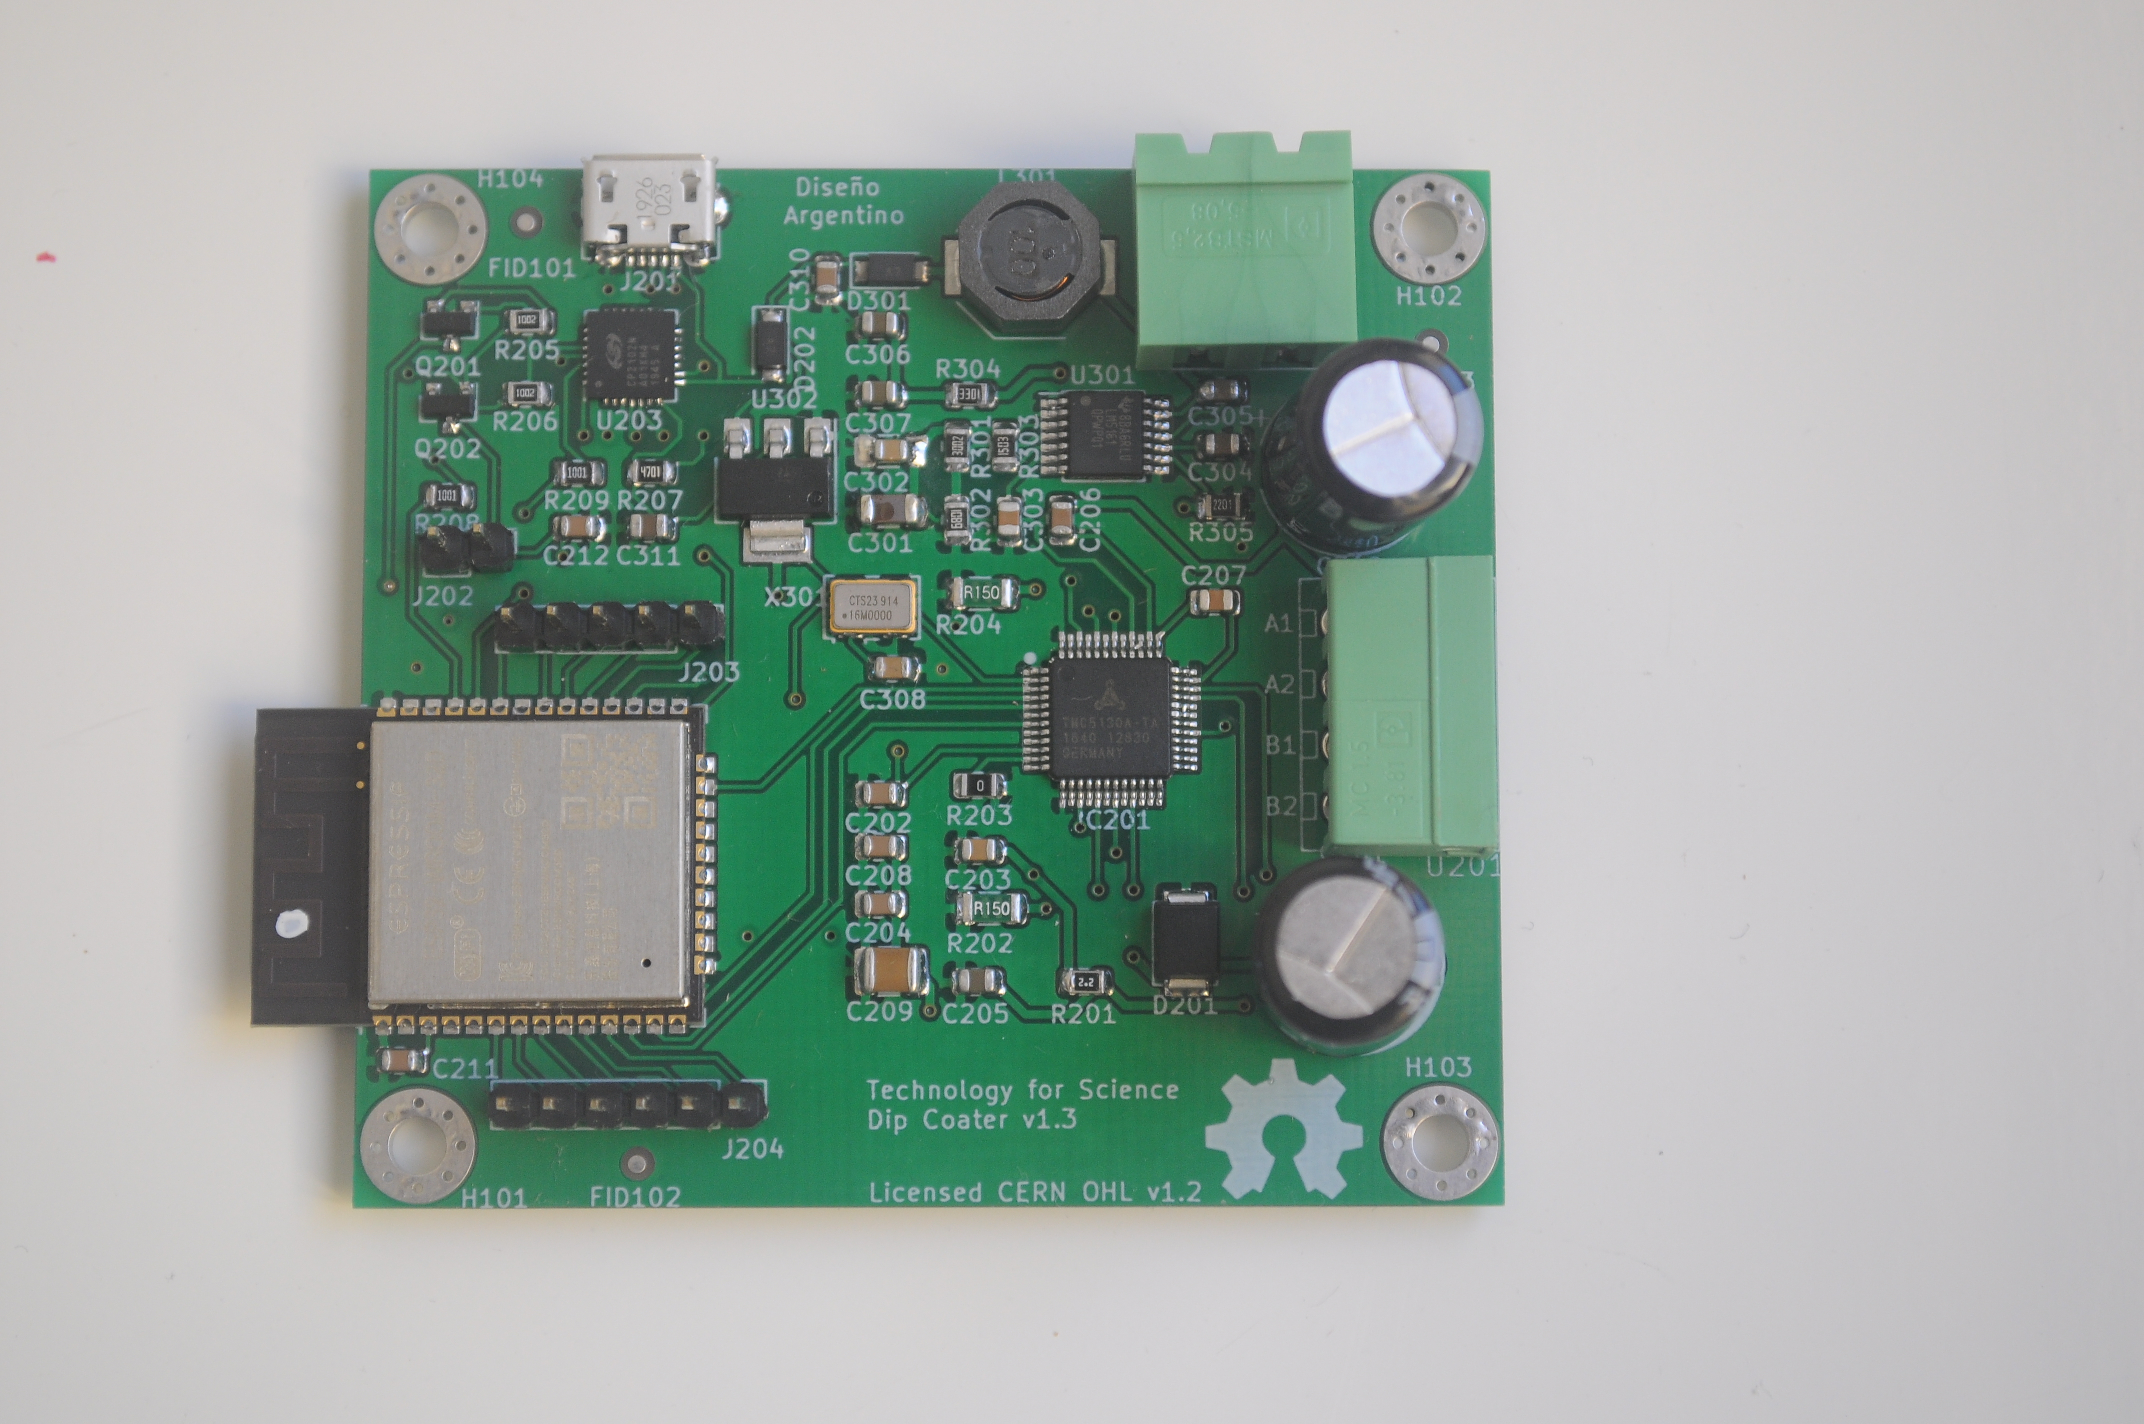
\includegraphics[width=.5\textwidth]{./Figures/dip_real_model.pdf}
	\caption{Placa fabricada MAYER SRL.}
	\label{fig:dip_real_model}
\end{figure}

%----------------------------------------------------------------------------------------
%	SECTION 2
%----------------------------------------------------------------------------------------

\section{Firmware}

\subsection{Capas de abstracción}
\subsection{Framework de trabajo}
\subsection{Módulos principales}



%----------------------------------------------------------------------------------------
%	SECTION 3
%----------------------------------------------------------------------------------------

\section{Estructura mecánica}
\subsection{Fabricación de piezas personalizadas a través de mecanizado CNC}

Como se menciono en la \ref{sec:estructura_mecanica} se utilizó para el software BOBCAD 

\begin{figure}[ht]
	\centering
	\includegraphics[width=.5\textwidth]{./Figures/3d_carro.png}
	\caption{Pieza personalizada para el carro.}
	\label{fig:carro}
\end{figure}

\begin{figure}[ht]
	\centering
	\includegraphics[width=.5\textwidth]{./Figures/3d_estrategia.png}
	\caption{Estrategias de mecanizado en software Bodcad.}
	\label{fig:estrategia}
\end{figure}

\begin{figure}[ht]
	\centering
	\includegraphics[width=.5\textwidth]{./Figures/3d_top.png}
	\caption{Piezas personalizado para sostener estructura superior.}
	\label{fig:estructura_superior}
\end{figure}

\subsection{Modelos 3D y real}

\begin{figure}[ht]
	\centering
	\includegraphics[width=.8\textwidth]{./Figures/3d.jpg}
	\caption{Modelo 3D.}
	\label{fig:mecanica_3d_model}
\end{figure}

\begin{figure}[ht]
	\centering
	\includegraphics[width=.5\textwidth]{./Figures/real.png}
	\caption{Primer prototipo dip coater TECSCI.}
	\label{fig:mecanica_real_model}
\end{figure}